\documentclass{article}  % Tipo di documento
\usepackage[utf8]{inputenc} % Per caratteri accentati
\usepackage[italian]{babel} % Lingua italiana
\usepackage{amsthm}
\usepackage{amssymb}
\usepackage{amsmath}  % simboli matematici avanzati
\usepackage{xcolor} % Per i colori
\usepackage{titlesec} % Per personalizzare i titoli
\usepackage{tikz}
\usetikzlibrary{mindmap,trees}
\usepackage[most]{tcolorbox}
\tcbuselibrary{theorems}
\usepackage{tikz}
\usetikzlibrary{automata, positioning, arrows}
\tcbuselibrary{breakable}
\usepackage{graphicx}
\graphicspath{ {./media/} }

\newtcbtheorem[no counter]{theorem}{Teorema}%
{colback=blue!5, 
colframe=blue!50!black, 
fonttitle=\bfseries,
    breakable,            % permette di spezzare il box su più pagine
    enhanced,
    break at=0pt}{}

\theoremstyle{definition}
\newtheorem{definition}{Definizione}[section]

% Imposto colore delle subsection
\titleformat{\subsection}
  {\normalfont\large\color{red}} % stile del titolo
  {\thesubsection}{1em}{} % numerazione e spaziatura

% Definiamo un nuovo ambiente per gli esempi
\newtcolorbox{esempio}[1][]{
    colback=white,       % colore di sfondo
    colframe=gray,       % colore del bordo
    fonttitle=\bfseries,
    title=#1,
    boxrule=0.5pt,       % spessore del bordo
    arc=4pt,             % angoli arrotondati
    left=4pt, right=4pt, top=4pt, bottom=4pt
}

\newtcolorbox{esercizio}[1][]{
    colback=white,       % colore di sfondo
    colframe=green!60!black,       % colore del bordo
    fonttitle=\bfseries,
    title=#1,
    boxrule=0.5pt,       % spessore del bordo
    arc=4pt,             % angoli arrotondati
    left=4pt, right=4pt, top=4pt, bottom=4pt,
    breakable,            % permette di spezzare il box su più pagine
    enhanced,
    break at=0pt
}

\newtcolorbox{osservazioni}[1][]{
    colback=white,       % colore di sfondo
    colframe=yellow!80!orange,       % colore del bordo
    fonttitle=\bfseries,
    title=#1,
    boxrule=0.5pt,       % spessore del bordo
    arc=4pt,             % angoli arrotondati
    left=4pt, right=4pt, top=4pt, bottom=4pt,
    breakable,            % permette di spezzare il box su più pagine
    enhanced,
    break at=0pt
}

% Creo un nuovo ambiente "ragionamento" senza quadratino
\newenvironment{ragionamento}[1][]
  {\begin{proof}[Ragionamento#1]\renewcommand{\qedsymbol}{}\normalfont}
  {\end{proof}}

\title{Informatica Teorica}
\author{Ede Boanini}
\date{\today}

\begin{document}
% genera automaticamente l’indice
\tableofcontents
\newpage % va a nuova pagina
\maketitle
%%%%%%%%%%%%%%%%%%%%%%%%%%%%%%%%%%%%%%%%%%%%%%%%%%%%%%%%%%%%%%%%%%%%%%%%%%%%%%%%%%%%%%%%%%%%%%%%%%%%%%
\section{Introduzione}
\subsection{Definizioni essenziali}
\begin{definition}[Grafo]
Sia \(G=(V,E)\) un grafo non orientato, dove:
\begin{itemize}
  \item \(V\) è l'insieme dei nodi
  \item \(E\) è l'insieme degli archi
\end{itemize}
\end{definition}
\begin{definition}[Coppia di nodi]
Siano \(u\) e \(v\) due nodi di un grafo \(G = (V,E)\). 
La coppia \(\{u,v\}\) rappresenta un arco che connette i nodi \(u\) e \(v\). 
\end{definition}
\begin{definition}[Grado di un nodo]
Numero di archi che collegano un nodo $v$ ad altri nodi.
\[
deg(v)=k
\]
\end{definition}
\begin{definition}[Grafo $k$-regolare]
Un grafo \(G=(V,E)\) è $k$-regolare se ogni nodo ha grado $k$:
\[
\forall v \in V, \quad deg(v)=k
\]
\end{definition}
%%%%%%%%%%%%%%%%%%%%%%%%%%%%%%%%%%%%%%%%%%%%%%%%%%%%%%%%%%%%%%%%%%%%%%%%%%%%%%%%%%%%%%%%%%%%%%%%%%%%%%
\subsection{Tipi di dimostrazioni}
\begin{tikzpicture}[
  level 1/.style={
    sibling distance=40mm, 
    level distance=20mm,
    every node/.append style={font=\small} % qui riduco il font dei figli
  },
  every node/.style={
    rectangle, draw, rounded corners, 
    align=center, 
    top color=blue!20, 
    bottom color=blue!10
  }
]
\node {Tipi di \\ dimostrazione}
  child {node {Per \\ costruzione}}
  child {node {Per \\ assurdo}}
  child {node {Per \\ induzione}};
\end{tikzpicture}

\begin{definition}[Dimostrazione per Costruzione]
Il teorema afferma che esiste un particolare tipo di oggetto. Un modo per dimostrare un teorema di questo tipo è mostrare come costruire l’oggetto.
\end{definition}
\(\bigstar\) Idea: vuoi dimostrare che un oggetto esiste? Lo costruisci direttamente.


\begin{esempio}[Esempio]
\footnotesize % riduce la dimensione del font
Per ogni numero pari $n>2$, \(\exists\) un grafo $3$-regolare con $n$ nodi.
\begin{proof}
Sia $n$ un numero pari maggiore di 2. Costruisco un grafo \(G=(V,E)\) con $n$ nodi come segue:\newline
Dispongo i nodi in cerchio. Collego ogni nodo con il successivo \(\{i,i+1\}\) formando un ciclo. Dopodichè collego ogni nodo con il suo opposto \(\{i,i+n/2\}\).
In questo modo, ogni nodo ha 3 archi, quindi $G$ è $3$-regolare. 
\end{proof}
Ho dimostrato il teorema costruendo un grafo che rispetta l'ipotesi (che il numero di nodi sia un numero pari maggiore di 2) arrivando poi alla tesi: ipotesi \(\rightarrow\) costruzione \(\rightarrow\) tesi.
\end{esempio}

\begin{definition}[Dimostrazione per Assurdo]
Assumo che il teorema sia falso e mostro che questa assunzione conduce a una proposizione che è logicamente impossibile, cioè che contraddice un fatto già dimostrato o una proprietà nota. Questa contraddizione implica che l’assunzione iniziale era falsa, quindi il teorema è vero.
\end{definition}
\(\bigstar\) Idea: supponi che il teorema sia falso (neghi la tesi). Se questa assunzione porta ad un'assurdità, allora il teorema deve essere vero. 

\begin{definition}[Dimostrazione per Induzione]
Metodo usato per mostrare che tutti gli elementi di un insieme infinito possiedono una proprietà specifica. Questa dimostrazione
consiste in due fasi:
\begin{itemize}
  \item \textbf{Base:} dimostro che la proprietà \(\mathcal{P}\) vale per il primo elemento dell'insieme. Verifico che $\mathcal{P}(1)$ (oppure $\mathcal{P}(0)$, dipende da dove parte l'insieme) è vera. 
  \item \textbf{Passo induttivo:} suppongo che, per ogni $k \geq 1$, la proprietà $\mathcal{P}(k)$ sia vera (ipotesi induttiva). Ciò implica che anche $\mathcal{P}(k+1)$ è vera.
\end{itemize}

\end{definition}
\(\bigstar\) Idea: dimostri che una proprietà vale per infiniti casi.
\begin{esempio}[Esempio]
\footnotesize % riduce la dimensione del font
Per ogni $t \geq 0$, vale la seguente formula: \newline
\[
P_t=PM^t-Y\Big(\frac{M^t-1}{M-1}\Big)
\]
\begin{proof}
\textbf{Base:} dimostra che la formula è vera per $t=0$.
\[
P_0=PM^0-Y\Big(\frac{M^0-1}{M-1}\Big)
\]
Sapendo che $P_0=P$ e $M^0=1$, dunque ottengo:
\[
P=P-Y\Big(\frac{0}{M-1}\Big)
\]
\[
P=P-Y(0)
\]
\[
P=P-0
\]
\[
P=P
\]
\textbf{Passo induttivo:} \(\forall{k}\geq0\), assumo che la formula è vera per $t=k$ (ipotesi induttiva), ovvero assumo vera che:
\begin{align*}
  P_k=PM^k-Y\Big(\frac{M^k-1}{M-1}\Big) \tag*{(ipotesi induttiva)}
\end{align*}
questo per dimostrare che:
\begin{align*}
  P_{k+1}=PM^{k+1}-Y\Big(\frac{M^{k+1}-1}{M-1}\Big) \tag*{(tesi)}
\end{align*}
Se riesco a dimostrare che per $t=k+1$ è vera, allora automaticamente è vera $\forall{t}\geq 0$.
Iniziamo:\newline
Per definizione so che,
\begin{align*}
  P_{k+1}=P_kM-Y
\end{align*}
usando l'ipotesi induttiva sostituisco
\begin{align*}
  P_{k+1}= \textcolor{red}{P_k} M-Y
\end{align*}
e ottengo
\begin{align*}
  P_{k+1}= \Big[\textcolor{red}{PM^k-Y\Big(\frac{M^k-1}{M-1}\Big)} \Big] M-Y
\end{align*}
sviluppando alla fine ottengo
\begin{align*}
  = PM^{k+1}-Y \Big(\frac{M^{k+1}-1}{M-1}\Big)
\end{align*}
Che è proprio quello che volevo dimostrare.
\end{proof}
Ho dimostrato il teorema utilizzando l'ipotesi induttiva (che supponevo vera, per questo posso applicarla) 
nella definizione di $P_{k+1}$, poi ho sviluppato ed ottenuto la tesi.
\end{esempio}
\begin{tabular}{|c|c|}
\hline
IPOTESI & Condizioni che si assumono vere \\ \hline
TESI & Ciò che bisogna dimostrare \\ \hline
\end{tabular}
\break
%%%%%%%%%%%%%%%%%%%%%%%%%%%%%%%%%%%%%%%%%%%%%%%%%%%%%%%%%%%%%%%%%%%%%%%%%%%%%%%%%%%%%%%%%%%%%%%%%%%%%%
\subsection{Macchina di Turing}
\begin{definition}[Macchina deterministica]
  Esiste una sola scelta possibile per ogni combinazione di stato e simbolo dell'alfabeto.
  \begin{esempio}[Esempio]
\footnotesize % riduce la dimensione del font

\begin{tikzpicture}[node distance=3cm, auto]
  \node[state, initial] (q1) {$q_1$};
  \node[state, accepting, right of=q1] (q2) {$q_2$};
  \node[state, right of=q2] (q3) {$q_3$};

  \draw 
  (q1) edge[loop above] node{1} (q1)
  (q1) edge[->, above] node{0} (q2)
  (q2) edge[loop above] node{1} (q2)
  (q2) edge[->, bend left, above] node{0} (q3)
  (q3) edge[->, bend left, below] node{0, 1} (q2);
\end{tikzpicture} \newline
Se sono nello stato $q_1$ e leggo il simbolo $0$ ho solo una scelta: cambiare stato in $q_2$.
\end{esempio}
\end{definition}

\begin{definition}[Macchina non deterministica]
  Esistono più scelte possibili per ogni combinazione di stato e simbolo dell'alfabeto.
  \begin{esempio}[Esempio]
\footnotesize % riduce la dimensione del font
\begin{tikzpicture}[node distance=3cm, auto]
  \node[state, initial] (q1) {$q_1$};
  \node[state, accepting, right of=q1] (q2) {$q_2$};
  \node[state, right of=q2] (q3) {$q_3$};

  \draw 
  (q1) edge[loop above] node{0} (q1)
  (q1) edge[->, above] node{0,1} (q2)
  (q2) edge[loop above] node{1} (q2)
  (q2) edge[->, bend left, above] node{0} (q3)
  (q3) edge[->, bend left, below] node{0, 1} (q2);
\end{tikzpicture} \newline
Se sono nello stato $q_1$ e leggo il simbolo $0$ ho più scelte:
\begin{itemize}
  \item cambiare stato in $q_2$
  \item tornare nello stato $q_1$
\end{itemize}
\end{esempio}
\end{definition}

\begin{definition}[Linguaggio]
  Insieme di stringhe costruite a partire da un alfabeto e che rispettano certe regole.
  \begin{esempio}[Esempio]
\footnotesize % riduce la dimensione del font
\begin{itemize}
  \item Sia l'alfabeto $\Sigma=\{0,1\}$
  \item Sia $L$ il linguaggio 
\end{itemize}
Linguaggio che contiene stringhe con un numero pari di 1:\newline
$L=\{11,011,0011,1100,0110,1111,01111,\dots\}$ 
\end{esempio}
\end{definition}

\begin{definition}[MdT modello standard] Una Macchina di Turing standard è una 7-upla
   $(Q,\Sigma,\Gamma,\delta,q_0,q_{accept}, q_{reject})$ dove $Q,\Sigma,\Gamma$ sono insiemi finiti e:
  \begin{itemize}
    \item $Q$ insieme degli stati
    \item $\Sigma$ alfabeto di input (non contiene il simbolo * blank); $\Sigma \subseteq \Gamma$
    \item $\Gamma$ alfabeto del nastro (tutti i simboli che può leggere e scrivere sul nastro, include anche il simbolo * blank)
    \item $\delta:Q\times\Gamma \rightarrow Q\times\Gamma\times\{S,D\}$ funzione di transizione
    \item $q_0 \in Q$ stato iniziale
    \item $q_{accept} \in Q$ è lo stato di accettazione
    \item $q_{reject} \in Q$ è lo stato di rifiuto dove $q_{accept} \neq q_{reject}$
  \end{itemize}
  Il modello standard è dunque una macchina deterministica.
\end{definition}

\begin{definition}[Linguaggio decidibile/ricorsivo]
  Un linguaggio $L$ è \textbf{decidibile} se $\exists$ una MdT $M$ tale che, per ogni stringa $w\in \Sigma^*$ in input:
  \begin{itemize}
    \item Se $w \in L \implies$ M si ferma (accettando $w$) nello stato $q_{accept}$; Quindi accetta la stringa.
    \item Se $w \notin L \implies$ M si ferma (rifiutando $w$) nello stato $q_{reject}$; Quindi rifiuta la stringa.
  \end{itemize}
Notare che la macchina si ferma sempre. In questo caso si dice che la macchina "decide" $L$.
\end{definition}

\begin{definition}[Linguaggio semidecidibile/ricorsivamente enumerabile]
    Un linguaggio $L$ è \textbf{semidecidibile} se $\exists$ una MdT $M$ tale che, per ogni stringa $w\in \Sigma^*$ in input:
  \begin{itemize}
    \item Se $w \in L \implies$ M si ferma (accettando $w$) nello stato $q_{accept}$; Quindi accetta la stringa.
    \item Se $w \notin L \implies$ M va in loop, non fermandosi mai.
  \end{itemize}
Notare che la macchina \underline{non} si ferma sempre. In questo caso si dice che la macchina "riconosce" $L$.
\end{definition}

\begin{definition}[Linguaggio indecidibile]
    Un linguaggio $L$ è \textbf{indecidibile} quando $\nexists$ una MdT $M$ in grado di decidere $L$. Ma può esistere una MdT in grado
    di riconoscere $L$.\\
    \textit{Nota: $L$ è indecidibile e potrebbe essere semidecidibile, ma mai decidibile.}
\end{definition}

\begin{definition}[Linguaggio di una macchina] 
  Se $A$ (linguaggio) è l'insieme di tutte le stringhe che la MdT $M$ accetta oppure riconosce, dico che $M$ accetta o riconosce $A$ e lo indico come $L(M)=A$. \newline
  Se $M$ non accetta nessuna stringa, lo indico come $L(M)=\emptyset$
\end{definition}

\begin{definition}[Enumeratore]
  Un enumeratore è una MdT che genera tutte le stringhe del linguaggio (separandole con il simbolo "$\#$"), 
  una dopo l'altra, senza ricevere nessun input. Infatti, la macchina $E$ inizia a lavorare su nastro vuoto (input vuoto). \newline \newline
  Funzionamento:
  \begin{enumerate}
    \item L'enumeratore viene eseguito inizialmente su nastro vuoto (nessun input)
    \item Genera la stringa scrivendola sul nastro
    \item Quando ha terminato di scrivere la stringa, la invia al dispostivo di output (stampante)
    \item Torna al passo 2
  \end{enumerate}
  
\end{definition}
\break
%%%%%%%%%%%%%%%%%%%%%%%%%%%%%%%%%%%%%%%%%%%%%%%%%%%%%%%%%%%%%%%%%%%%%%%%%%%%%%%%%%%%%%%%%%%%%%%%%%%%%%
%%%%%%%%%%%%%%%%%%%%%%%%%%%%%%%%%%%%%%%%%%%%%%%%%%%%%%%%%%%%%%%%%%%%%%%%%%%%%%%%%%%%%%%%%%%%%%%%%%%%%%
\section{Decidibilità}
\begin{tikzpicture}[
  level 1/.style={
    sibling distance=40mm, 
    level distance=20mm,
    every node/.append style={font=\small} % qui riduco il font dei figli
  },
  every node/.style={
    rectangle, draw, rounded corners, 
    align=center, 
    top color=blue!20, 
    bottom color=blue!10
  }
]
\node {Linguaggio}
  child {node {Decidibile}}
  child {node {Semidecidibile}}
  child {node {Indecidibile}};
\end{tikzpicture}\newline \newline
Come provare che un linguaggio è decidibile, semidecidibile o indecidibile?
\begin{itemize}
  \item $L$ è decidibile: dimostrazione per costruzione
  \item $L$ è semidecidibile: dimostrazione per costruzione
  \item $L$ è indecidibile: dimostrazione per assurdo + riduzione ad un problema che sappiamo essere indecidibile (es: Teorema dell'arresto) oppure Teorema di Rice
\end{itemize}
\begin{definition}[Codifica di una MdT] La notazione $R(M)$ indica la codifica di una macchina. Spesso utilizzata nelle dimostrazioni.
\end{definition}
\subsection{Decidibilità}
Questa dimostrazione fa riferimento ad un automa a stati finiti deterministico (DFA). Lo stesso quesito per una MdT non è decidibile (vedi esercizio 2.2).
Lo scopo è mostrare come funziona la dimostrazione per costruzione.
\begin{esercizio}[Esercizio 1.1]
\footnotesize % riduce la dimensione del font
Sia il linguaggio $L_{DFA} = \{(R(M), w) \mid M \text{ accetta } w\}$. Dimostrare che $L$ è decidibile.
\begin{ragionamento}
$L_{DFA}$ è l'insieme delle codifiche di automi a stati finiti deterministici che accettano $w$. Ovvero, siano $M_1$,$M_2$,$M_3$ tre DFA:
\begin{itemize}
  \item $M_1$ accetta $w$, allora $R(M_1) \in L_{DFA}$
  \item $M_2$ rifiuta $w$, allora $R(M_2) \notin L_{DFA}$
  \item $M_3$ accetta $w$, allora $R(M_3) \in L_{DFA}$
\end{itemize}
Quindi \(L_{DFA}=\{R(M_1),R(M_3)\}\) \newline
**utilizzo dimostrazione per costruzione.
\end{ragionamento}
\begin{proof}
\begin{align*}
  L_{DFA} = \{(R(M), w) \mid M \text{ accetta } w\} \tag*{(ipotesi)}
\end{align*}
\begin{align*}
  L_{DFA} \text{è decidibile} \tag*{(tesi)}
\end{align*}
  Sapendo che per ipotesi $L_{DFA} = \{(R(M), w) \mid M \text{ accetta } w\}$, allora costruisco una MdT $N$ che decide $L_{DFA}$.
  Dato in input $(R(M),w)$, dove $R(M)$ è la codifica di un DFA arbitrario e $w$ una stringa:
  \begin{enumerate}
    \item Controlla che $R(M)$ sia una codifica valida e che $w$ sia una stringa, altrimenti rifiuta.
    \item Simula $M$ su input $w$.
    \item Se la simulazione termina:
    \begin{itemize}
      \item in uno stato accettante $\implies N$ termina accettando $R(M)$; \\ Quindi $R(M) \in L_{DFA}$
      \item in uno stato di rifiuto $\implies N$ termina rifiutando $R(M)$; \\ Quindi $R(M) \notin L_{DFA}$
    \end{itemize}
  \end{enumerate}
  Ho costruito una macchina $N$ in grado di decidere $L_{DFA}$; Inoltre, poichè un DFA ha
  un numero di stati finiti e la stringa $w$ è finita, la simulazione termina in uno stato finale 
  (accettante o di rifiuto), garantendo che anche $N$ si fermi sempre accettando o rifiutando l'input. 
  Pertanto, si dimostra che $L_{DFA}$ è decidibile.
 \end{proof}
\end{esercizio}
%%%%%%%%%%%%%%%%%%%%%%%%%%%%%%%%%%%%%%%%%%%%%%%%%%%%%%%%%%%%%%%%%%%%%%%%%%%%%%%%
\subsection{Indecidibilità}
Un linguaggio $L$ è indecidibile quando $\nexists$ una MdT in grado di fermarsi sempre accettando o rifiutando l'input. Ciò vuol dire che:
\begin{itemize}
  \item $L$ è indecidibile e anche semidecidibile
  \item $L$ è indecidibile ma non semidecidibile
\end{itemize}
Pertanto, quando viene richiesto di dimostrare l'indecidibilità di un linguaggio:
\begin{itemize}
  \item Se sospetto che $L$ possa essere indecidibile $+$ semidecidibile, allora:
  \begin{enumerate}
    \item Applico la dimostrazione per costruzione; 
   
  cioè, costruisco una MdT che riconosce\footnote{Turing-reconizable: MdT si ferma accettando le stringhe che appartengono al linguaggio e va in loop
  per quelle che non appartengono.} il linguaggio. 
   \item Effettuo la riduzione ad un linguaggio noto indecidibile. 
  \end{enumerate}
  Nel primo punto dimostro la semidecidibilità di $L$ e nel secondo la indecidibilità.
  \item Se sospetto che il linguaggio è indecidibile ma non semidecidibile, allora posso considerare una di queste tecniche:
  \begin{center}
      \begin{tikzpicture}[
  level 1/.style={
    sibling distance=30mm, 
    level distance=20mm,
    every node/.append style={font=\small} % qui riduco il font dei figli
  },
  every node/.style={
    rectangle, draw, rounded corners, 
    align=center, 
    top color=blue!20, 
    bottom color=blue!10
  }
]
\node {Dimostrare indecidibilità}
  child {node {dim assurdo \\ + riduzione}}
  child {node {riduzione diretta}}
  child {node {teorema di Rice}}
  child {node {diagonalizzazione}};
\end{tikzpicture}
  \end{center}

  \begin{itemize}
    \item dimostrazione per assurdo + effettuo la riduzione ad un linguaggio noto indecidibile
    \item riduzione diretta 
    \item uso il Teorema di Rice
    \item applico la diagonalizzazione
  \end{itemize}
\end{itemize}

\subsection{Esercizi}
\begin{theorem}{}
  SSia il linguaggio $L = \{(R(M), w) \mid M \text{ accetta } w\}$. Dimostrare che $L$ è semidecidibile ma anche indecidibile.
\end{theorem}
\begin{esercizio}[Esercizio 2.1]
\footnotesize % riduce la dimensione del font
Sia il linguaggio $L_1 = \{(R(M), w) \mid M \text{ accetta } w\}$. Dimostrare che $L$ è semidecidibile.
\begin{ragionamento}
$L_1$ è l'insieme delle codifiche di MdT che accettano $w$. Ovvero, siano $M_1$,$M_2$,$M_3$ tre MdT:
\begin{itemize}
  \item $M_1$ accetta $w$, allora $R(M_1) \in L_1$
  \item $M_2$ rifiuta $w$, allora $R(M_2) \notin L_1$
  \item $M_3$ accetta $w$, allora $R(M_3) \in L_1$
\end{itemize}
Quindi \(L_1=\{R(M_1),R(M_3)\}\)  \\
Dato che devo dimostrare la semidecidibilità di $L_1$, costruisco una MdT che riconosce il linguaggio. 
\end{ragionamento}
\begin{proof}
\begin{align*}
  L_1 = \{(R(M), w) \mid M \text{ accetta } w\} \tag*{(ipotesi)}
\end{align*}
\begin{align*}
  L_1 \text{ è semidecidibile} \tag*{(tesi)}
\end{align*}
  Costruisco una MdT $N$ che riconosce $L_1$.
  Dato in input $(R(M),w)$, dove $R(M)$ è la codifica di una MdT arbitraria e $w$ una stringa, la MdT $N$ si comporta come segue:
  \begin{enumerate}
    \item Controlla che $R(M)$ sia una codifica valida e che $w$ sia una stringa, altrimenti rifiuta.
    \item Simula $M$ su input $w$.
    \item Se la simulazione termina:
    \begin{itemize}
      \item in uno stato accettante $\implies N$ termina accettando $R(M)$; \\ Quindi $R(M) \in L_1$
      \item in uno stato di rifiuto $\implies N$ termina rifiutando $R(M)$; \\ Quindi $R(M) \notin L_1$
    \end{itemize}
  \end{enumerate}
  Notare che la macchina $N$ va in loop sull'input $(R(M),w)$ se $M$ va in loop su $w$. \\
  Un decisore deve \underline{sempre} fermarsi (in ogni caso), ma qui, se $M$ va in loop su $w$, $N$ non si fermerà mai. 
  Questo rende $N$ un riconoscitore e non un decisore. \\
  Ho dimostrato che $L_1$ è semidecidibile costruendo la MdT $N$ che riconosce tale linguaggio.
  Pertanto, si dimostra che $L_1$ è semidecidibile.
 \end{proof}
\end{esercizio}

\begin{esercizio}[Esercizio 2.2]
\footnotesize % riduce la dimensione del font
Sia il linguaggio $L_1 = \{(R(M), w) \mid M \text{ accetta } w\}$. Dimostrare che $L$ è indecidibile.
\begin{ragionamento}
Per dimostrarlo, applico:
\begin{itemize}
  \item Dim per assurdo (suppongo per assurdo (nego la tesi) per poi ottenere una contraddizione, che rende falsa l'assunzione fatta)
\end{itemize}
\end{ragionamento}
\begin{proof}
\begin{align*}
  L_1 = \{(R(M), w) \mid M \text{ accetta } w\} \tag*{(ipotesi)}
\end{align*}
\begin{align*}
  L_1 \text{ è indecidibile} \tag*{(tesi)}
\end{align*}
Per applicare la dimostrazione per assurdo nego la tesi, quindi suppongo per assurdo che $L_1$ sia decidibile.
  Sapendo che per ipotesi (la mia per assurdo, non quella del teorema) $L_1$ è decidibile, allora $\exists$ una MdT $N$ che decide $L_1$ con il seguente funzionamento:
\[
N(R(M),w) =
\begin{cases}
\text{accept} & \text{se } M \text{ accetta } w\\
\text{reject} & \text{se } M \text{ non accetta } w
\end{cases}
\]
Con "non accetta" si intende che $M$ potrebbe rifiutare $w$ oppure andare in loop.\\
  Dato in input $(R(M),w)$ alla MdT $N$, dove $R(M)$ è la codifica di una MdT arbitraria e $w$ una stringa:
  \begin{enumerate}
    \item $N$ controlla che $R(M)$ sia una codifica valida e che $w$ sia una stringa, altrimenti rifiuta.
    \item Simula $M$ su input $w$.
    \item Se la simulazione termina:
    \begin{itemize}
      \item in uno stato accettante $\implies N$ termina accettando $R(M)$; \\ Quindi $R(M) \in L_1$
      \item in uno stato di rifiuto/va in loop $\implies N$ termina rifiutando $R(M)$; \\ Quindi $R(M) \notin L_1$
    \end{itemize}
  \end{enumerate}
Adesso costruisco una nuova MdT $D$ con $N$ come subroutine. $D$ chiama $N$ per determinare cosa fa $M$ quando l'input per $M$ è la sua 
stessa codifica (e non la stringa $w$). Il comportamento di $D$ è l'opposto di $N$, ovvero:
\[
D(R(M)) =
\begin{cases}
\text{accept} & \text{se } M \text{ non accetta } R(M)\\
\text{reject} & \text{se } M \text{  accetta } R(M)
\end{cases}
\]
Funzionamento di $D$:
\begin{enumerate}
\item Esegue $N$ su input $(R(M),R(M))$ dove $R(M)$ è la codifica della MdT M:
\begin{itemize}
    \item Se $N$ si ferma accettando $\implies$ $D$ rifiuta.\\
    (ricorda che se $N$ accetta allora vuol dire che $M$ ha accettato $R(M)$)
    \item Se $N$ si ferma rifiutando $\implies$ $D$ accetta. \\
    (ricorda che se $N$ rifiuta allora vuol dire che $M$ non ha accettato $R(M)$)
\end{itemize} 
\end{enumerate}
Cosa succederebbe se fornissimo alla MdT $D$ la propria codifica come input? Otterrei:
\[
D(R(D)) =
\begin{cases}
\text{accept} & \text{se } D \text{ non accetta } R(D)\\
\text{reject} & \text{se } D \text{  accetta } R(D)
\end{cases}
\]
che è una contraddizione.\\
\textbf{Conclusione:} Poiché abbiamo ottenuto una contraddizione ($D$ rifiuta $R(D)$ quando $D$ accetta $R(D)$), l’ipotesi che $L_1$ sia decidibile è falsa. Pertanto, $L_1$ è indecidibile.
 \end{proof}
\end{esercizio}

\begin{theorem}{}
  SSia il linguaggio $L = \{(R(M), w) \mid M \text{ accetta } w\}$. Dimostrare che $\overline{L}$ non è semidecidibile.
\end{theorem}
\begin{esercizio}[Esercizio 2.3]
  \footnotesize % riduce la dimensione del font
Sia il linguaggio $L_1 = \{(R(M), w) \mid M \text{ accetta } w\}$. Dimostrare che $\overline{L_1}$ non è semidecidibile.
\begin{ragionamento}
  Devo dimostrare che $\overline{L_1}=\{(R(M), w) \mid M \text{ non accetta } w\}$ non è semidecidibile, ovvero che $\nexists$ una MdT in grado 
  di riconoscere $\overline{L_1}$. Procedo per assurdo.
\end{ragionamento}
\begin{proof}
  \begin{align*}
  L_1 = \{(R(M), w) \mid M \text{ accetta } w\} \tag*{(ipotesi)}
\end{align*}
\begin{align*}
  \overline{L_1} \text{ non è semidecidibile} \tag*{(tesi)}
\end{align*}

  Sappiamo che $L_1$ è un linguaggio semidecidibile (esercizio 2.1). \\
  Suppongo per assurdo che anche $\overline{L_1}$ sia semidecidibile (nego la tesi, ipotesi per assurdo). 
  Dato che $L_1, \overline{L_1}$ sono entrambi semidecidibili $\implies$ per definizione, $L_1$ è decidibile. Ma questo è assurdo perchè abbiamo dimostrato
  che $L_1$ è indecidibile (esercizio 2.2). Ciò porta ad una contraddizione e l'ipotesi che $\overline{L_1}$ sia semidecidibile è falsa. 
  Pertanto, $\overline{L_1}$ è non semidecidibile. 

\end{proof}
\end{esercizio}
\break
\subsection{Famosi problemi indecidibili}
\subsubsection{Halting Problem}
\begin{definition}(Problema dell'arresto)
  Esiste una MdT $H$ che preso in input $(M,w)$, termina dicendo:
  \begin{itemize}
    \item Sì, se $M$ termina su $w$ 
    \item No, se $M$ va in loop su $w$
  \end{itemize}
  Tale macchina esiste? No.
\end{definition}
\begin{definition}(Linguaggio Halting Problem) Sia $\mathcal{L}_{\text{Halt}}$ il linguaggio del problema dell'arresto definito come segue:
  \begin{align*}
    \mathcal{L}_{\text{Halt}} = \{(R(M),w) \mid M \text{ termina su } w\}
  \end{align*}
  Notare che $\mathcal{L}_{\text{Halt}}$ è semidecidibile, ovvero $\exists$ una MdT $N$ che dato in input $(R(M),w)$:
  \begin{itemize}
    \item Se $M$ termina su $w$, allora $N$ accetta \\ (Se $M$ termina su $w \implies (R(M),w) \in \mathcal{L}_{\text{Halt}}$)\footnote{Ho scritto
     "$M$ termina su $w$" e non "$w \in L(M)$" poichè si sta parlando di terminare su $w$ e non accettare $w$. La dicitura 
    classica $w \in L(M)$ si scrive solo quando $M$ accetta $w$.}. 
    \item Se $M$ non termina su $w$, allora $N$ va in loop
  \end{itemize}
    *Attenzione: "$M$ termina su $w$" e non dice "$M$ accetta $w$", che sono due cose differenti.
  Se $M$ termina su $w$, allora $N$ accetta; ovvero l'importante è che $M$ termini su $w$, che sia in uno stato accettante o di rifiuto. (Quindi non ci interessa
  se $M$ accetta o rifiuta $w$, quello che ci interessa è che $M$ si fermi su $w$.) \\ \\
  Pertanto, $\exists$ una MdT che riconosce (ma non decide) $\mathcal{L}_{\text{Halt}}$.
\end{definition}

\begin{osservazioni}[Osservazione]
\footnotesize % riduce la dimensione del font
Il problema dell'arresto (o, equivalentemente, il linguaggio 
$\mathcal{L}_{\text{Halt}}$) è \textbf{indecidibile}, cioè non esiste una MdT che
termina sempre dando la risposta corretta. 
Tuttavia, $\mathcal{L}_{\text{Halt}}$ è \textbf{semidecidibile}: esiste infatti una MdT universale che, dato in input 
$(R(M),w)$, termina accettando se $M$ termina su $w$, mentre può non
terminare se $M$ non termina su $w$.
\end{osservazioni}

Il problema dell'arresto è semidecidibile + indecidibile, oppure, equivalentemente scrivo:
\begin{align*}
  \textcolor{red}{\mathcal{L}_{\text{Halt}} \text{ è semidecidibile ma non decidibile}}
\end{align*}

\begin{theorem}{Halting Problem (2.4.1)} 
  IIl problema dell'arresto è indecidibile. \\
  $\mathcal{L}_{\text{Halt}} = \{(R(M),w) \mid M \text{ termina su } w\}$ è indecidibile.
  \footnotesize % riduce la dimensione del font
  \begin{proof}
    \begin{align*}
      \mathcal{L}_{\text{Halt}} = \{(R(M),w) \mid M \text{ termina su } w\} \tag*{(ipotesi)}
    \end{align*}
    \begin{align*}
      \mathcal{L}_{\text{Halt}} \text{ è indecidibile} \tag*{(tesi)}
    \end{align*}
    Suppongo per assurdo che il problema dell'arresto sia decidibile (ipotesi per assurdo, nego la tesi).
    Quindi, per ipotesi, $\exists$ una MdT $H$ che risolve il problema dell'arresto. \\
    $H$ su input ($R(M),w$) dove $R(M)$ è la codifica di una MdT arbitraria e $w$ una stringa:
    \begin{itemize}
      \item Se $M$ termina su $w$, allora $H$ accetta
      \item Se $M$ non termina su $w$, allora $H$ rifiuta
    \end{itemize}
    Modifico la MdT $H$ per costruire $H'$ con il seguente 
    comportamento. 
    \[
    H'(R(M),w) =
    \begin{cases}
      \text{loop} & \text{se } M \text{ termina su } w\\
      \text{reject} & \text{se } M \text{  non termina su } w
    \end{cases}
    \]
    $H'$ su input ($R(M),w$): 
    \begin{itemize}
      \item Se $M$ termina su $w$, allora $H'$ va in loop
      \item Se $M$ non termina su $w$, allora $H'$ rifiuta
    \end{itemize}
    Adesso costruisco un'altra MdT $D$ (che prende in input solo la codifica di una macchina)\footnote{invece dell'input
     ($R(M),w$), prende in input ($R(M)$)} 
    combinando $H'$ con una procedura. 
    \[
    D(R(M)) =
    \begin{cases}
      \text{loop} & \text{se } M \text{ termina su } R(M)\\
      \text{reject} & \text{se } M \text{  non termina su } R(M)
    \end{cases}
    \]
    La macchina $D$ su input ($R(M)$):
    \begin{enumerate}
      \item Controlla che $R(M)$ sia un codifica valida, altrimenti rifiuta
      \item Esegue varie transizioni che, a partire dall'input, produce la coppia ($R(M),R(M)$) \\
      (legge la codifica della macchina in input e la copia come secondo argomento da fornire a $H'$)
      \item Esegue $H'$ sull'input ($R(M),R(M)$):
      \begin{itemize}
        \item Se $H'$ va in loop, allora anche $D$ va in loop \\
        (ricorda che se $H'$ va in loop vuol dire che $M$ ha terminato su $R(M)$)
        \item Se $H'$ rifiuta, allora $D$ rifiuta \\
        (ricorda che se $H'$ rifiuta vuol dire che $M$ non ha mai terminato su $R(M)$)
      \end{itemize}
    \end{enumerate}
  E adesso cosa succederebbe se fornissi alla MdT $D$ la propria codifica come input? Otterrei:
    \[
    D(R(D)) =
    \begin{cases}
      \text{loop} & \text{se } D \text{ termina su } R(D)\\
      \text{reject} & \text{se } D \text{  non termina su } R(D)
    \end{cases}
    \]
    una contraddizione. \\
    \textbf{Conclusione:} Poichè ho ottenuto una contraddizione ($D$ va in loop su $R(D)$ $\iff$ $D$ termina su $R(D)$), l'ipotesi
    che il problema dell'arresto sia decidibile è falsa. Pertanto, il problema dell'arresto è indecidibile (oppure scrivo: 
    Pertanto, $\mathcal{L}_{\text{Halt}}$ è indecidibile).
  \end{proof}
\end{theorem}
\begin{theorem}{}
  I $\mathcal{L}_{\text{Halt}}$ è semidecidibile. 
  $\overline{\mathcal{L}_{\text{Halt}}}$ non è semidecidibile.
  \footnotesize % riduce la dimensione del font
  \begin{proof}
    Sappiamo per definizione, che $\mathcal{L}_{\text{Halt}}$ è semidecidibile. \\
    Suppongo per assurdo che $\overline{\mathcal{L}_{\text{Halt}}}$ sia anch'esso semidecidibile. Dato che
    $\overline{\mathcal{L}_{\text{Halt}}}$,$\mathcal{L}_{\text{Halt}}$ sono entrambi semidecidibili $\implies$ per
    definizione, $\mathcal{L}_{\text{Halt}}$ è decidibile. Ma questo è assurdo perchè abbiamo dimostrato che 
    $\mathcal{L}_{\text{Halt}}$ è indecidibile (teorema 2.4.1). Ciò porta ad una contraddizione e l'ipotesi che $\overline{\mathcal{L}_{\text{Halt}}}$
    sia semidecidibile è falsa. \\ Pertanto, $\overline{\mathcal{L}_{\text{Halt}}}$ è non semidecidibile. 
  \end{proof}
\end{theorem}

\subsubsection{Problema del nastro vuoto}
\begin{definition}[Problema del nastro vuoto]
  Esiste una MdT $E$ che preso in input $R(M)$, termina dicendo:
  \begin{itemize}
    \item Sì, se $M$ termina su nastro vuoto
    \item No, se $M$ non termina su nastro vuoto
  \end{itemize}
  Tale macchina esiste? No. \\
  \footnotesize % riduce la dimensione del font
  *Attenzione: "termina su nastro vuoto" significa "termina quando parte su nastro vuoto".
\end{definition}
\begin{definition}[Linguaggio Blank-Tape Halting Problem]
  Sia $\mathcal{L}_{\text{Blank-Tape}}$ il linguaggio del problema del nastro vuoto definito come segue:
  \begin{align*}
    \mathcal{L}_{\text{Blank-Tape}} = \{R(M) \mid M \text{ termina su nastro vuoto}\}
  \end{align*}
  Notare che $\mathcal{L}_{\text{Blank-Tape}}$ è semidecidibile.
\end{definition}
Quindi, il problema del nastro vuoto è semidecidibile + indecidibile, oppure, equivalentemente scrivo:
\begin{align*}
  \textcolor{red}{\mathcal{L}_{\text{Blank-Tape}} \text{ è semidecidibile ma non decidibile}}
\end{align*}


\begin{theorem}{Blank-Tape Halting Problem (versione A: DA RIVEDERE)}
IIl problema del nastro vuoto è indecidibile. \\
$\mathcal{L}_{\text{Blank-Tape}} = \{R(M) \mid M \text{ termina su nastro vuoto}\}$ è indecidibile.
\footnotesize % riduce la dimensione del font
  \begin{ragionamento}
  Per dimostrarlo, uso la dim per assurdo e poi effettuo una riduzione da un problema noto indecidibile (es: problema dell'arresto) al mio (problema del nastro vuoto). \\
  Dato che sto ragionando per assurdo, non posso usare questa: se $A \leq_m B$ $\;\wedge\;$ $A$ è indecidibile $\implies$ $B$ è indecidibile (teorema 3.2); ma devo usare 
  questa: se $A \leq_m B$ $\;\wedge\;$ $B$ è decidibile $\implies$ $A$ è decidibile (teorema 3.1); \\
  Quindi costruisco una riduzione del tipo: $\mathcal{L}_{\text{Halt}} \leq_m \mathcal{L}_{\text{Blank-Tape}}$.
  \end{ragionamento}
  \begin{proof}
    \begin{align*}
      \mathcal{L}_{\text{Blank-Tape}} = \{R(M) \mid M \text{ termina su nastro vuoto}\} \tag*{(ipotesi)}
    \end{align*}
    \begin{align*}
      \mathcal{L}_{\text{Blank-Tape}} \text{ è indecidibile} \tag*{(tesi)}
    \end{align*}
    Siano $\mathcal{L}_{\text{Halt}}$ , $\mathcal{L}_{\text{Blank-Tape}}$ due linguaggi su $\Sigma_H^*$, $\Sigma_B^*$ rispettivamente, dove:
    \begin{itemize}
      \item $\mathcal{L}_{\text{Halt}}$ è il linguaggio del problema dell'arresto
      \item $\mathcal{L}_{\text{Blank-Tape}}$ è il linguaggio del problema del nastro vuoto
    \end{itemize}
    \textcolor{red}{1. Ipotesi per assurdo} \\
    Suppongo per assurdo che $\mathcal{L}_{\text{Blank-Tape}}$ sia decidibile (ipotesi per assurdo). Quindi per ipotesi $\exists$ una MdT $E$ 
    che decide $\mathcal{L}_{\text{Blank-Tape}}$. Ovvero:
    \[
    E(R(M)) =
    \begin{cases}
      \text{accept} & \text{se } M \text{ termina su nastro vuoto} \\
      \text{reject} & \text{se } M \text{  non termina su nastro vuoto}
    \end{cases}
    \]
    \textcolor{red}{2. Costruisco funzione di riduzione} \\
    Costruisco una funzione di riduzione $f: \Sigma_H^* \rightarrow \Sigma_B^*$ t.c. $\forall{w} \in \Sigma_H^*$:
    \begin{align*}
      w \in \mathcal{L}_{\text{Halt}} \iff f(w) \in \mathcal{L}_{\text{Blank-Tape}}
    \end{align*}
    Quindi, costrusco la funzione di riduzione (che sarebbe la MdT $R$):
    \begin{itemize}
      \item Se $w$ non è della forma $(R(M),w)$, pongo $f(w)=1$
      \item Se $w=(R(M),w)$, allora pongo $f(w)=R(M')$
    \end{itemize}
    Ovvero, il funzionamento della MdT $R$ è costruire una nuova macchina $M'$, praticamente il seguente:
    \begin{enumerate}
      \item $R$ riceve come input $w=(R(M),w)$ da $N$
      \item $R$ costruisce la nuova macchina $M'$ che ha questo comportamento:
      \begin{enumerate}
        \item $M'$ viene avviata su nastro vuoto (condizione del Blank-Tape Halting Problem)
        \item $M'$ scrive $w$ sul nastro
        \item $M'$ riporta la testina all'inizio del nastro
        \item $M'$ esegue $M$ su $w$
      \end{enumerate}
      \item $R$ genera l'output $R(M')$ (che è la nuova macchina costruita nel passo 2)
    \end{enumerate}
    \textcolor{red}{3. Costruisco MdT che decide il problema dell'arresto} \\
    Adesso, costrusco una MdT $N$ che decide $\mathcal{L}_{\text{Halt}}$:
    \begin{enumerate}
      \item $N$ su input $w \in \Sigma_H^*$ calcola $f(w) \in \Sigma_B^*$
      \item $N$ esegue $E$ su $f(w)$:
      \begin{itemize}
        \item Se $E$ accetta, allora $N$ accetta \\
        (ricorda che se $E$ accetta, vuol dire che $M'$ ha terminato su nastro vuoto (se $M'$ termina su nastro vuoto, vuol
        dire che $M$ ha terminato su $w$))
        ovvero: Se $R(M') \in \mathcal{L}_{\text{Blank-Tape}}$, allora $(R(M),w) \in \mathcal{L}_{\text{Halt}}$ \\
        ma è più corretto scrivere: \\
        $w \in \mathcal{L}_{\text{Halt}} \iff  f(w) \in \mathcal{L}_{\text{Blank-Tape}}$
        \item Se $E$ rifiuta, allora $N$ rifiuta \\
        (ricorda che se $E$ rifiuta, vuol dire che $M'$ non ha terminato su nastro vuoto (se $M'$ non termina su nastro vuoto (loop), vuol
        dire che $M$ non ha terminato su $w$ (loop))) \\ 
        ovvero: Se $R(M') \notin \mathcal{L}_{\text{Blank-Tape}}$, allora $(R(M),w) \notin \mathcal{L}_{\text{Halt}}$ \\
        ma è più corretto scrivere: \\
        $w \notin \mathcal{L}_{\text{Halt}} \iff f(w) \notin \mathcal{L}_{\text{Blank-Tape}}$
      \end{itemize} 
    \end{enumerate}
  Quindi $N$ è un algoritmo di decisione per il problema dell'arresto che applica la funzione di riduzione per ogni input e sfrutta
  la MdT $E$ che decide $\mathcal{L}_{\text{Blank-Tape}}$ per decidere $\mathcal{L}_{\text{Halt}}$. Perchè alla fine $N$ si ferma
  accettando $w$ se e solo se $E$ si ferma accettando $f(w)$ oppure $N$ si ferma
  rifiutando $w$ se e solo se $E$ si ferma rifiutando $f(w)$. \\
  La costruzione e il funzionamento della MdT $N$ rende il problema dell'arresto decidibile. Ma questo è assurdo perchè sappiamo
  che il problema dell'arresto è indecidibile, quindi questo porta ad una contraddizione. Poichè ho ottenuto una contraddizione, l'ipotesi 
  che il problema del nastro vuoto sia decidibile è falsa. Pertanto, il problema del nastro vuoto è indecidibile. 
  \end{proof}
  Disegno: \\
    \begin{center}
    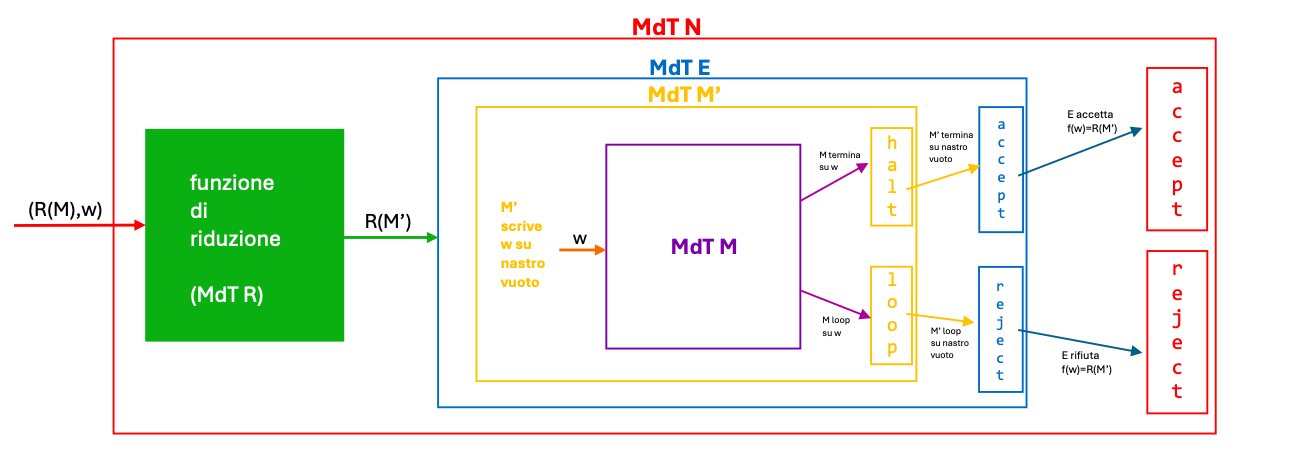
\includegraphics[width=0.9\linewidth]{BTHP.png}
  \end{center}
\end{theorem}

\begin{theorem}{Blank-Tape Halting Problem (versione B)}
IIl problema del nastro vuoto è indecidibile. \\
$\mathcal{L}_{\text{Blank-Tape}} = \{R(M) \mid M \text{ termina su nastro vuoto}\}$ è indecidibile.
\footnotesize % riduce la dimensione del font
  \begin{ragionamento}
    Per dimostrarlo, \underline{non} uso la dim per assurdo ma effettuo \textbf{direttamente} una riduzione dal problema dell'arresto al mio. Ovvero, 
    costruisco una riduzione del tipo: $\mathcal{L}_{\text{Halt}} \leq_m \mathcal{L}_{\text{Blank-Tape}}$. \\
    Uso solo la riduzione perchè "sfrutto":
    \begin{enumerate}
      \item La definizione di funzione di riduzione\\
      ($L_1 \leq_m L_2$ se $\exists$ una funzione di riduzione $f: \Sigma_1^* \rightarrow \Sigma_2^*$ t.c. $\forall{w}\in \Sigma_1^*$: \\
      $w \in L_1 \iff f(w) \in L_2$
      )
      \item Il teorema $A \leq_m B$ $\;\wedge\;$ $A$ è indecidibile $\implies$ $B$ è indecidibile (teorema 3.2).
    \end{enumerate}
  \end{ragionamento}
  \begin{proof}
        \begin{align*}
      \mathcal{L}_{\text{Blank-Tape}} = \{R(M) \mid M \text{ termina su nastro vuoto}\} \tag*{(ipotesi)}
    \end{align*}
    \begin{align*}
      \mathcal{L}_{\text{Blank-Tape}} \text{ è indecidibile} \tag*{(tesi)}
    \end{align*}
    Siano $\mathcal{L}_{\text{Halt}}$ , $\mathcal{L}_{\text{Blank-Tape}}$ due linguaggi su $\Sigma_H^*$, $\Sigma_B^*$ rispettivamente, dove:
    \begin{itemize}
      \item $\mathcal{L}_{\text{Halt}}$ è il linguaggio del problema dell'arresto
      \item $\mathcal{L}_{\text{Blank-Tape}}$ è il linguaggio del problema del nastro vuoto
    \end{itemize}
    
    Sia $\mathcal{L}_{\text{Halt}} = \{(R(M),w) \mid M \text{ termina su } w\}$.
    È noto che $\mathcal{L}_{\text{Halt}}$ è indecidibile. \\
    \textcolor{red}{1. Riduzione} \\
    Definisco una funzione di riduzione\footnote{ricorda la funzione di riduzione trasforma un'istanza del problema dell'arresto H in un'istanza del problema del nastro vuoto B}
     $f: \Sigma_H^* \rightarrow \Sigma_B^*$ come segue. \\
    Dato in input $(R(M),w)$\footnote{istanza del problema dell'arresto}  la funzione $f$ genera come output $R(M')$\footnote{istanza del problema del nastro vuoto}, 
    dove $M'$ è la nuova MdT costruita dalla funzione di riduzione $f$ che ha questo comportamento:
    \begin{enumerate}
      \item $M'$ inizia la computazione su nastro vuoto
      \item $M'$ scrive $w$ sul nastro
      \item $M'$ riporta la testina all'inzio del nastro
      \item $M'$ esegue $M$ su $w$
    \end{enumerate}
    La funzione di riduzione $f$ trasforma ogni istanza del problema dell'arresto $(R(M),w)$
    in un'istanza $R(M')$ del problema del nastro vuoto, dove $M'$ inizia la computazione su nastro vuoto, scrive $w$ sul nastro ed esegue $M$ su $w$.  
    Per definizione di funzione di riduzione, vale:
    \[
    (R(M),w) \in \mathcal{L}_{\text{Halt}} \iff f((R(M),w)) \in \mathcal{L}_{\text{Blank-Tape}}.\footnote{dove $f((R(M),w))=R(M')$; precisando che $w=(R(M),w)$ e $f(w)=R(M')$
    dove $w$ è l'input dato alla funzione di riduzione e $f(w)$ è l'ouput generato dalla stessa funzione di riduzione, ovvero il valore ottenuto applicando $f$ a $w$.}
    \]  
    Poiché $\mathcal{L}_{\text{Halt}} \leq_m \mathcal{L}_{\text{Blank-Tape}}$ e $\mathcal{L}_{\text{Halt}}$ è indecidibile, segue che $\mathcal{L}_{\text{Blank-Tape}}$ è indecidibile.
  \end{proof}
\end{theorem}


\subsubsection{Problema del Linguaggio Vuoto}
\begin{theorem}{Emptiness Problem}
IIl problema del linguaggio vuoto è indecidibile. \\
$\mathcal{L}_{\text{Emptiness}} = \{R(M) \mid L(M)= \emptyset \}$ è indecidibile.
\footnotesize % riduce la dimensione del font
  \begin{ragionamento}
    Per dimostrarlo, uso la dim per assurdo + costruisco una riduzione dal problema dell'arresto al mio, ovvero 
    $\mathcal{L}_{\text{Halt}} \leq_m \mathcal{L}_{\text{Emptiness}}$. \\ Uso quindi la MdT E che decide $\mathcal{L}_{\text{Emptiness}}$ per decidere
    $\mathcal{L}_{\text{Halt}}$. Uso solo la riduzione perchè "sfrutto":
    \begin{enumerate}
      \item La definizione di funzione di riduzione\\
      ($L_1 \leq_m L_2$ se $\exists$ una funzione di riduzione $f: \Sigma_1^* \rightarrow \Sigma_2^*$ t.c. $\forall{w}\in \Sigma_1^*$: \\
      $w \in L_1 \iff f(w) \in L_2$
      )
      \item Il teorema $A \leq_m B$ $\;\wedge\;$ $B$ è decidibile $\implies$ $A$ è decidibile (teorema 3.1).
    \end{enumerate}
  \end{ragionamento}
  \begin{proof}
        \begin{align*}
      \mathcal{L}_{\text{Emptiness}} = \{R(M) \mid L(M)= \emptyset \} \tag*{(ipotesi)}
    \end{align*}
    \begin{align*}
      \mathcal{L}_{\text{Emptiness}} \text{ è indecidibile} \tag*{(tesi)}
    \end{align*}
    Siano $\mathcal{L}_{\text{Halt}}$ , $\mathcal{L}_{\text{Emptiness}}$ due linguaggi su $\Sigma_H^*$, $\Sigma_E^*$ rispettivamente, dove:
    \begin{itemize}
      \item $\mathcal{L}_{\text{Halt}}$ è il linguaggio del problema dell'arresto
      \item $\mathcal{L}_{\text{Emptiness}}$ è il linguaggio dell'emptiness problem
    \end{itemize}
    \textcolor{red}{1. Ipotesi per assurdo} \\
    Suppongo per assurdo che $\mathcal{L}_{\text{Emptiness}}$ sia decidibile (ipotesi per assurdo). Allora $\exists$ una MdT $E$ che decide $\mathcal{L}_{\text{Emptiness}}$.
    Ovvero:
    \[
    E(R(M)) =
    \begin{cases}
      \text{accept} & \text{se } M \text{ non accetta nessuna stringa} \\
      \text{reject} & \text{se } M \text{  accetta almeno una stringa}
    \end{cases}
    \]
    \textcolor{red}{2. Riduzione} \\
    Definisco una funzione di riduzione\footnote{ricorda la funzione di riduzione trasforma un'istanza del problema dell'arresto H in un'istanza dell'emptiness problem E}
     $f: \Sigma_H^* \rightarrow \Sigma_E^*$ come segue. \\
    Dato in input $(R(M),w)$\footnote{istanza del problema dell'arresto}  la funzione $f$ genera come output $R(M')$\footnote{istanza del problema dell'emptiness problem}, 
    dove $M'$ è la nuova MdT costruita dalla funzione di riduzione $f$ che ha il seguente comportamento ($R(M)$ è la codifica di una MdT arbitraria
    e $w$ una stringa). \\ \\ $M'$ su una stringa di input $x$ generica:
    \begin{itemize}
      \item se $x \neq w$, rifiuta
      \item se $x = w$, esegue $M$ su $w$ dove:
      \begin{itemize}
        \item se $M$ accetta $w$, allora $M'$ accetta $w$ (perchè $x=w$)
        \item se $M$ rifiuta $w$, allora $M'$ rifiuta $w$
        \item se $M$ va in loop su $w$, allora $M'$ va in loop
      \end{itemize}
    \end{itemize}
    In sostanza, osservandolo dal punto di vista del linguaggio accettato da $M'$:
    \[
    L(M') =
    \begin{cases}
      \{w\} & \text{se } M \text{ accetta } w\\
      \emptyset & \text{se } M \text{ rifiuta } w \text{ o se non termina (loop) su } w
    \end{cases}
    \]
    \textcolor{red}{3. Costruisco MdT che decide il problema dell'arresto} \\
    Adesso, costrusco una MdT $N$ che decide $\mathcal{L}_{\text{Halt}}$:
    \begin{enumerate}
      \item $N$ su input $w \in \Sigma_H^*$ calcola $f(w) \in \Sigma_E^*$ (riduzione)
      \item $N$ esegue $E$ su $f(w)$:
      \begin{itemize}
        \item Se $E$ accetta, allora $N$ rifiuta \\
        (se $E$ accetta, vuol dire che $M'$ ha linguaggio vuoto, cioè $M'$ ha rifiutato $w$, quindi $L(M')=\emptyset$ (se $M'$ rifiuta $w$, vuol
        dire che $M$ ha riufiutato $w$)) \\
        ovvero: Se $R(M') \in \mathcal{L}_{\text{Emptiness}}$, allora $(R(M),w) \notin \mathcal{L}_{\text{Halt}}$ \\
        ma è più corretto scrivere: \\
        $w \notin \mathcal{L}_{\text{Halt}} \iff  f(w) \in \mathcal{L}_{\text{Emptiness}}$
        \item Se $E$ rifiuta, allora $N$ accetta \\
        (se $E$ rifiuta, vuol dire che $M'$ \underline{non} ha linguaggio vuoto, cioè $M'$ ha accettato $w$, quindi $L(M')=\{w\}$ (se $M'$ accetta $w$, vuol
        dire che $M$ ha accettato $w$)) \\ 
        ovvero: Se $R(M') \notin \mathcal{L}_{\text{Emptiness}}$, allora $(R(M),w) \in \mathcal{L}_{\text{Halt}}$ \\
        ma è più corretto scrivere: \\
        $w \in \mathcal{L}_{\text{Halt}} \iff f(w) \notin \mathcal{L}_{\text{Emptiness}}$
      \end{itemize} 
    \end{enumerate}
    *Precisando che $w=(R(M),w)$ e $f(w)=R(M')$
    dove $w$ è l'input dato alla funzione di riduzione e $f(w)$ è l'ouput generato dalla stessa funzione di riduzione, ovvero il valore ottenuto applicando $f$ a $w$. \\

    Poiché $\mathcal{L}_{\text{Halt}} \leq_m \mathcal{L}_{\text{Emptiness}}$ e $\mathcal{L}_{\text{Emptiness}}$ è decidibile (ipotesi per assurdo), segue 
    che $\mathcal{L}_{\text{Halt}}$ è decidibile.
    Ma questo è assurdo perché è ben noto che $\mathcal{L}_{\text{Halt}}$ è indecidibile (contraddizione). Poichè ho ottenuto una contraddizione, l'ipotesi che 
    $\mathcal{L}_{\text{Emptiness}}$ sia decidibile è falsa. Pertanto, l'emptiness problem è indecidibile.
  \end{proof}
\end{theorem}







\subsubsection{Problema dell'Equivalenza dei Linguaggi Accettati da due MdT}
\subsubsection{Problema della terminazione totale}
\subsection{Proprietà non banali delle MdT}
\subsubsection{Teorema di Rice}
\subsubsection{Problema del linguaggio vuoto}
\subsubsection{Problema della finitezza del linguaggio}
\subsubsection{Problema della terminazione di programmi su tutti gli input}

%%%%%%%%%%%%%%%%%%%%%%%%%%%%%%%%%%%%%%%%%%%%%%%%%%%%%%%%%%%%%%%%%%%%%%%%%%%%%%%%%%%%%%%%%%%%%%%%%%%%%%
%%%%%%%%%%%%%%%%%%%%%%%%%%%%%%%%%%%%%%%%%%%%%%%%%%%%%%%%%%%%%%%%%%%%%%%%%%%%%%%%%%%%%%%%%%%%%%%%%%%%%%
\break
%%%%%%%%%%%%%%%%%%%%%%%%%%%%%%%%%%%%%%%%%%%%%%%%%%%%%%%%%%%%%%%%%%%%%%%%%%%%%%%%%%%%%%%%%%%%%%%%%%%%%%
%%%%%%%%%%%%%%%%%%%%%%%%%%%%%%%%%%%%%%%%%%%%%%%%%%%%%%%%%%%%%%%%%%%%%%%%%%%%%%%%%%%%%%%%%%%%%%%%%%%%%%
\section{Riducibilità}
Ricorda la notazione $f$: input $\rightarrow$ output
\begin{definition}[Funzione di riduzione]
  Sia $L_1$,$L_2$ due linguaggi su $\Sigma_{1}^*,\Sigma_{2}^*,$ rispettivamente.
  Si dice che $L_1$ è riducibile a $L_2$, e si scrive \textcolor{red}{$L_1 \leq_{m} L_2$} se $\exists$ una funzione computabile totale
  $f:\Sigma^*_1 \rightarrow \Sigma^*_2$ chiamata \textbf{funzione di riduzione} t.c. $\forall{w}\in \Sigma^*_1$
  \begin{align*}
    w \in L_1 \iff f(w) \in L_2
  \end{align*}
  Spiegazione informale:\\
  Per effetturare una riduzione da $L_1$ a $L_2$, deve esistere una MdT $R$ (macchina di riduzione) che prende in input 
  una qualunque stringa $w \in \Sigma^*_1$ e la trasforma in una stringa $f(w) \in \Sigma^*_2$. 
  Ovvero, se la MdT $R$ prende in input un'istanza di $L_1$ allora produce come output un'istanza di $L_2$. \\
  La MdT $R$ calcola la funzione di riduzione $f$. \\
  In questo modo, se avessimo una MdT che decide $L_2$, potremmo decidere $L_1$ applicando $f$.
\end{definition} 
\begin{theorem}{3.1}
  SSe $A \leq_m B$ e $B$ è decidibile $\implies A$ è decidibile. 
\end{theorem}
\begin{esercizio}[Dimostrazione 3.1]
  \footnotesize % riduce la dimensione del font
  Se $A \leq_m B$ e $B$ è decidibile $\implies A$ è decidibile. 
  \begin{ragionamento}
    $A$,$B$ sono due linguaggi su $\Sigma^*_A$,$\Sigma^*_B$ rispettivamente. \\
    Per ipotesi: 
\begin{itemize}
  \item $A \leq_m B$, quindi $\exists$ una funzione di riduzione (totale e calcolabile da una MdT) da $A$ a $B$.
  \item $B$ è decidibile, quindi $\exists$ una MdT che decide $B$.
\end{itemize}
Dimostro che A è decidibile costruendo una MdT che decide A.
  \end{ragionamento}
  \begin{proof}
    \begin{align*}
  & A \leq_m B \;\wedge\; B \text{ è decidibile} \tag*{(ipotesi)}
\end{align*}
\begin{align*}
  A \text{ è decidibile} \tag*{(tesi)}
\end{align*}
Per ipotesi, posso definire $M$ la MdT di decisione per B e $f:\Sigma^*_A \rightarrow \Sigma^*_B$ la funzione di riduzione da $A$ a $B$ (calcolabile dalla MdT R). \\
Costruisco la MdT $N$ che decide A:
\begin{enumerate}
  \item $N$ su input $w \in \Sigma^*_A$, calcola $f(w) \in \Sigma^*_B$ \\
  ($N$ esegue $R$ su $w$ che effettua la riduzione producendo come output $f(w)$)
  \item $N$ esegue $M$ su $f(w)$:
  \begin{itemize}
    \item Se $M$ accetta $f(w)$, allora $N$ accetta $w$. \\
    $f(w) \in B \iff w \in A$
    \item Se $M$ rifiuta $f(w)$, allora $N$ rifiuta $w$.  \\
    $f(w) \notin B \iff w \notin A$ 
  \end{itemize}
\end{enumerate}
\textbf{{Conclusione:}} Ho costruito un algoritmo di decisione per $A$ che applica la riduzione per ogni input e sfrutta la MdT che 
decide $B$ per $A$. Inoltre, la MdT $N$ si arresta sempre per ogni input $w$, perchè $f$ è una funzione totale computabile 
(la funzione di riduzione) e $M$ è un algoritmo di decisione (MdT che si ferma per ogni input) per B.\\
Pertanto, A è decidibile.

  \end{proof}
  *Notare che scrivo "accetta" o "rifiuta" e non "termina in uno stato accettante" o "termina in uno stato di rifiuto" perchè
ho indicato "costruisco la MdT $N$ che decide A" e una MdT che decide un linguaggio si ferma per ogni input, quindi sarebbe ridondante
scriverlo. \\ \\
Spiegazione extra della dimostrazione: \\
Ovvero, la macchina $N$ ha due MdT al suo interno (prima esegue $R$ e poi $M$): 
\begin{itemize}
  \item MdT R che effettua la riduzione da A a B: 
  \begin{enumerate}
    \item $R$ riceve in input $w$ (istanza di $A$)
    \item $R$ effettua la riduzione; calcola la funzione di riduzione su $w$ (applica $f$ a $w$ che scrivo come $f(w)$)
    \item $R$ produce come output $f(w)$ (istanza di $B$)
  \end{enumerate}
  \item MdT $M$ che decide $B$:
  \begin{enumerate}
    \item $M$ riceve in input $f(w)$ 
    \item Se la computazione di $M$ termina:
    \begin{itemize}
      \item in uno stato accettante, allora $f(w) \in B$ 
      \item in uno stato di rifiuto, allora $f(w) \notin B$ 
    \end{itemize}
  \end{enumerate}
\end{itemize}
Quindi, $N$ termina accettando $w$ se e solo se $M$ termina accettando $f(w)$. Oppure, $N$ termina rifiutando $w$ se e solo se $M$ termina 
rifiutando $f(w)$.
Come ben sappiamo, $M$ decide solo istanze di $B$, per questo è necessario trasformare un'istanza di $A$ in una di $B$. 
La riduzione serve perchè $M$ non può ricevere un'istanza di $A$ ma solo di $B$ (perchè per ipotesi $B$ è decidibile e $M$ è
la macchina di decisione per $B$), quindi è necessario che "qualcuno" effettui la trasformazione, che è proprio quello che fa la MdT $R$.\\
Potendo trasformare un'istanza di $A$ in $B$ e sapendo che $B$ è decidibile allora posso "decidere" $A$.
\end{esercizio}

\begin{theorem}{3.2}
  SSe $A \leq_m B$ e $A$ è indecidibile $\implies B$ è indecidibile. 
\end{theorem}
\begin{esercizio}[Dimostrazione 3.2]
    \footnotesize % riduce la dimensione del font
    Se $A \leq_m B$ e $A$ è indecidibile $\implies B$ è indecidibile.
    \begin{ragionamento}
      Per dimostarlo, suppongo per assurdo che $B$ sia decidibile (nego la tesi, ipotesi per assurdo) e poi applico
      la riduzione e poi le definizioni che mi porteranno ad una contraddizione che rende falsa la mia ipotesi per assurdo
      rendendo poi vero il teorema.
    \end{ragionamento}
    \begin{proof}
        \begin{align*}
        & A \leq_m B \;\wedge\; A \text{ è indecidibile} \tag*{(ipotesi)}
      \end{align*}
      \begin{align*}
        B \text{ è indecidibile} \tag*{(tesi)}
      \end{align*}
      Suppongo per assurdo che $B$ sia decidibile (ipotesi per assurdo). \\
      Quindi per ipotesi $\exists$ una MdT $M$ che decide $B$. Inoltre, per ipotesi (del teorema), $\exists$ una funzione
      di riduzione $f: \Sigma^*_A \rightarrow \Sigma^*_B$ t.c. $\forall{w} \in \Sigma^*_A$:
      \begin{align*}
        w \in A \iff f(w) \in B
      \end{align*}
      Costruisco una MdT $N$ che decide $A$:
      \begin{enumerate}
        \item $N$ su input $w \in \Sigma^*_A$ calcola $f(w) \in \Sigma^*_B$
        \item $N$ esegue $M$ su $f(w)$:
        \begin{itemize}
          \item Se $M$ accetta, allora $N$ accetta \\ 
          (Se $f(w) \in B$, allora $w \in A$)
          \item Se $M$ rifiuta, allora $N$ rifiuta \\
          (Se $f(w) \notin B$, allora $w \notin A$)
        \end{itemize}
      \end{enumerate}
      Ho costruito un algoritmo di decisione per $A$. Ma quindi se $A \leq_m B$ e $B$ è decidibile, allora per definizione
      (teorema 3.1) $A$ è decidibile. Ma questo è assurdo (contraddizione) perchè $A$ è indecidibile (secondo l'ipotesi del teorema). 
      Poichè abbiamo ottenuto una contraddizione, l'ipotesi che $B$ sia decidibile è falsa. Pertanto, $B$ è indecidibile.
    \end{proof}
\end{esercizio}


\begin{theorem}{3.3}
  SSe $A \leq_m B$ e $B$ è semidecidibile $\implies A$ è semidecidibile. 
\end{theorem}
\begin{theorem}{3.4}
  SSe $A \leq_m B$ e $A$ non è semidecidibile $\implies B$ non è semidecidibile. 
\end{theorem}

\section{Complessità Temporale}
\subsection{P}
\subsubsection{Famosi problemi}
\subsection{NP}
\subsubsection{NP-Difficile}
\subsubsection{NP-Completo}
\subsubsection{Famosi problemi}
\section{Complessità Spaziale}
\end{document}
